\documentclass[11pt]{article}

% ==== Paquetes ====
\usepackage[utf8]{inputenc}
\usepackage[spanish]{babel}
\usepackage{amsmath, amssymb, amsfonts, siunitx}
\usepackage{graphicx}
\usepackage{float}
\usepackage{listings} % Para código
\usepackage{xcolor}
\usepackage{hyperref}
\usepackage{caption}
\usepackage{subcaption}
\usepackage{geometry}
\usepackage{tikz}

\geometry{margin=2.5cm}

% ==== Configuración de listings (para código) ====
\lstset{
  basicstyle=\ttfamily\small,
  numbers=left,
  numberstyle=\tiny,
  stepnumber=1,
  numbersep=5pt,
  backgroundcolor=\color{gray!10},
  frame=single,
  tabsize=2,
  breaklines=true,
  showstringspaces=false,
  keywordstyle=\color{blue},
  commentstyle=\color{green!50!black},
  stringstyle=\color{red!70!black}
}

% ==== Datos de la tarea ====
\title{IEE3682 - Electro-óptica \\
Tarea 1}
\author{Nicolás Seguel}
\date{Agosto 2025}

\begin{document}
\maketitle

% ==== Ejemplo de respuesta con texto y fórmulas ====
\section*{Pregunta 1}

Asumiendo que la esfera de zafiro se comporta como una lente gruesa de dos superficies esféricas, se utiliza la ecuación de lentes gruesas para determinar la distancia focal efectiva y la distancia entre la superficie de la esfera y la faceta de cada fibra.

\[
\Phi = \frac{(n-1)}{R_1} - \frac{(n-1)}{R_2} + \frac{(n-1)^2 d}{n R_1 R_2},
\]

donde:
\begin{itemize}
    \item $n$ es el índice de refracción del material,
    \item $R_1, R_2$ son los radios de curvatura de las superficies,
    \item $d$ es el espesor de la lente.
\end{itemize}

La longitud focal efectiva está dada por:
\[
f_{\text{eff}} = \frac{1}{\Phi}.
\]

Para una esfera de radio $R$:

\begin{itemize}
    \item La primera superficie tiene radio $R_1 = +R$ (convexa).
    \item La segunda superficie tiene radio $R_2 = -R$ (cóncava, ya que la luz entra por la otra cara).
    \item El espesor de la lente es el diámetro de la esfera, $d = 2R$.
\end{itemize}

Sustituyendo en la ecuación:

\[
\Phi = \frac{(n-1)}{R} - \frac{(n-1)}{-R} + \frac{(n-1)^2 (2R)}{n R (-R)}.
\]

\[
\Phi = \frac{2(n-1)}{R} - \frac{2(n-1)^2}{nR}.
\]

\[
\Phi = \frac{2(n-1)}{R}\left(1 - \frac{(n-1)}{n}\right).
\]

\[
\Phi = \frac{2(n-1)}{nR}.
\]

Por lo tanto, la longitud focal efectiva es:

\[
f_{\text{eff}} = \frac{1}{\Phi} = \frac{nR}{2(n-1)}.
\]

Para un radio $R = 1~\text{mm}$ y un índice $n = 1.76$:

\[
f_{\text{eff}} = \frac{1.76 \times 1~\text{mm}}{2(0.76)} \approx 1.158~\text{mm}.
\]

Ahora considerando que la fibra óptica debe estar posicionada en el foco de la lente, la distancia entre la superficie de la esfera y la faceta de cada fibra es:

\[
\text{BFL} = f_{\text{eff}} - R = 1.158~\text{mm} - 1~\text{mm} \approx 0.158~\text{mm}.
\]

\section*{Pregunta 2}

Un observador mira a través del fondo hacia adentro de un recipiente que contiene un gradiente de solución de azúcar y agua, muy concentrada en el fondo y menos concentrada en la superficie.

\begin{figure}[H]
  \centering
  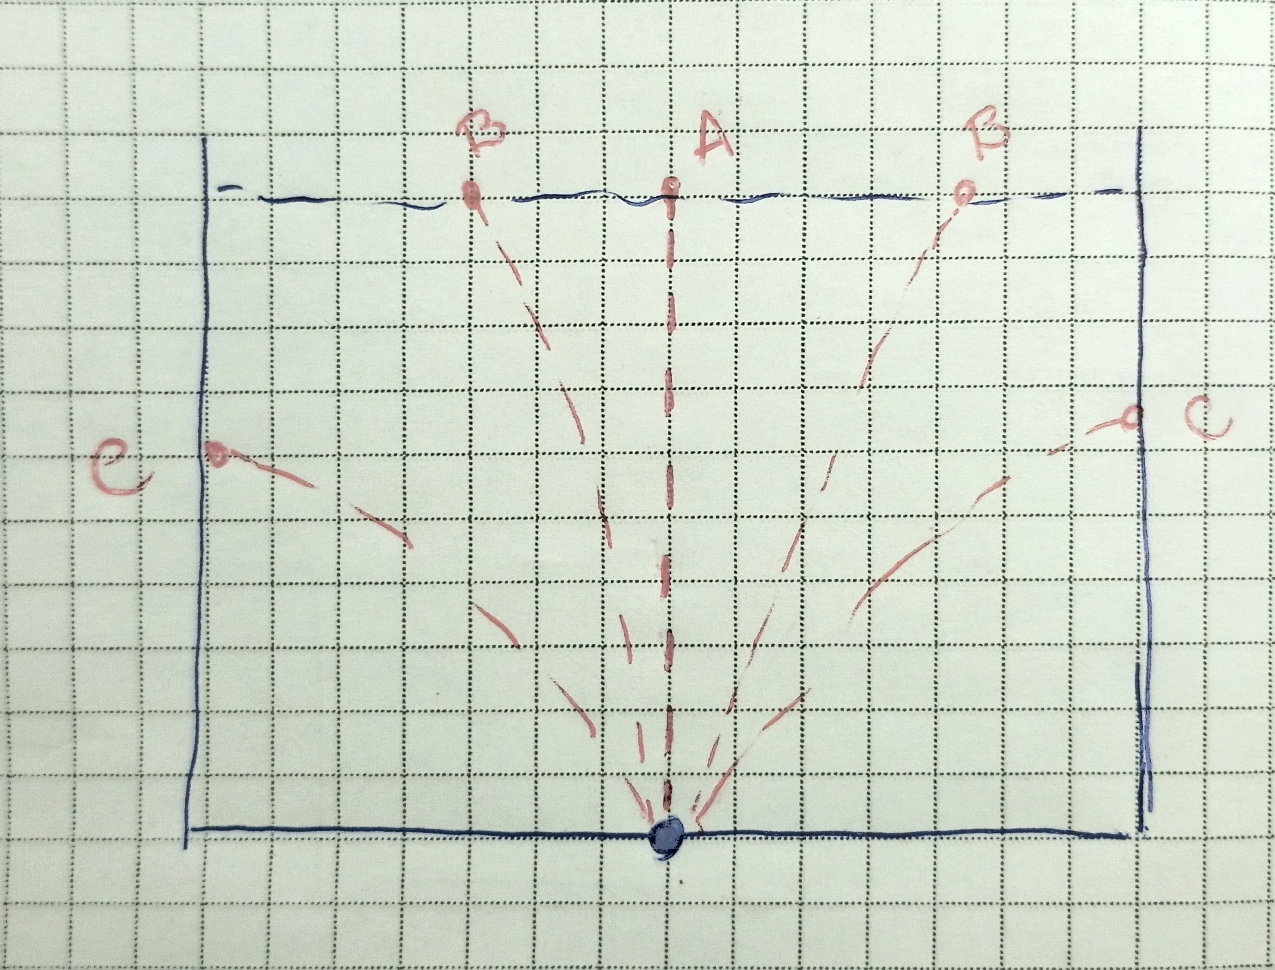
\includegraphics[width=0.7\textwidth]{p2.jpg}
  \caption{Trayectoria de un rayo de luz en un medio con índice de refracción variable.}
\end{figure}

La figura muestra las distintas trayectorias que puede seguir un rayo de luz al entrar en el recipiente. Los distintos rayos que llegan al ojo del observador son:

\begin{itemize}
  \item \textbf{Rayo A:} Entra perpendicularmente a la superficie del líquido y no se desvía.
  \item \textbf{Rayo B:} Entra con un ángulo pequeño y se desvía ligeramente hacia la normal al entrar en el líquido, debido al aumento del índice de refracción. La trayectoria curva del rayo genera una pequeña distorisión en la imagen observada.
  \item \textbf{Rayo C:} Entra con un ángulo mayor y puede venir de un lado del recipiente. Al entrar en el líquido, se desvía más hacia la normal y sigue una trayectoria curva más pronunciada. Este rayo puede generar una distorsión significativa en la imagen, haciendo que los objetos parezcan estar en posiciones diferentes a las reales.
\end{itemize}

Los rayos que recibe el observador tienen una distancia angular menor que la distancia angular real de los objetos dentro del recipiente, debido a la refracción y curvatura de las trayectorias. Esto provoca que los objetos parezcan estar más cerca del observador, con un efecto de magnificación. Además, la distorsión causada por la variación del índice de refracción y las trayectorias curvas puede hacer que los objetos parezcan deformados o desplazados de sus posiciones reales.

\section*{Pregunta 3}

Los telescopios de Kepler y Galileo son dos tipos de telescopios refractores que utilizan lentes para ampliar la imagen de objetos distantes. Ambos sistemas son afocales, lo que significa que los rayos de luz paralelos que entran en el sistema salen también como rayos paralelos, pero con un cambio en el ángulo y por ende en la magnificación angular.

Para modelar ambos telescopios, consideramos dos lentes delgadas: el objetivo (lente primaria) y el ocular (lente secundaria). La distancia entre las lentes es \(d\) y la distancia entre el observador y el ocular es \(z\). La distancia focal del objetivo es \(f_o\) y la del ocular es \(f_e\).

Para una lente delgada se tiene matriz:

\[L(f) = \begin{pmatrix} 1 & 0 \\ -\frac{1}{f} & 1 \end{pmatrix}\]

Para el espacio libre de propagación de longitud \(d\):

\[T(d) = \begin{pmatrix} 1 & d \\ 0 & 1 \end{pmatrix}\]

Para un telescopio refractor, la matriz total del sistema es:

\[M = T(z) \cdot L(f_e) \cdot T(d) \cdot L(f_o)\]

\subsection*{Matrices de los telescopios}

En el telescopio de Kepler, ambas lentes son convergentes, por lo que \(f_o > 0\) y \(f_e > 0\). La distancia entre las lentes es \(d = f_o + f_e\). Por lo que la matriz total es:

\[
M_{\text{Kepler}} = \begin{pmatrix} -\frac{f_e}{f_o} & f_e + f_o - \frac{f_o \cdot z}{f_e} \\ 0 & -\frac{f_o}{f_e} \end{pmatrix}
\]

En el telescopio de Galileo, el objetivo es convergente (\(f_o > 0\)) y el ocular es divergente (\(f_e < 0\)). La distancia entre las lentes es \(d = f_o - |f_e|\). La matriz total es:

\[
M_{\text{Galileo}} = \begin{pmatrix} \frac{f_e}{f_o} & f_o - f_e + \frac{f_o \cdot z}{f_e} \\ 0 & \frac{f_o}{f_e} \end{pmatrix}
\]

Se tiene que \(m = f_o / f_e\) es la magnificación angular del telescopio. Por lo que las matrices pueden reescribirse en función de \(m\):

\[
M_{\text{Kepler}} = \begin{pmatrix} -\frac{1}{m} & f_e(m + 1) - m \cdot z \\ 0 & -m \end{pmatrix}
\]
\[
M_{\text{Galileo}} = \begin{pmatrix} \frac{1}{m} & f_e(m - 1) + m \cdot z \\ 0 & m \end{pmatrix}
\]

\subsection*{Características comunes y diferencias}

\begin{itemize}
  \item \(\mathbf{C=0}\) en ambas matrices. Esto indica que los rayos entrantes paralelos salen paralelos.
  \item \(\mathbf{D}\) es la magnificación angular, es decir, la razón entre el ángulo de salida y el ángulo de entrada para rayos paralelos. Su valor es \(m = f_o/f_e\), pero con signo diferente: negativo en Kepler (imagen invertida) y positivo en Galileo (imagen erguida).
  \item \(\mathbf{A}\) es la magnificación lateral para rayos que no son paralelos a la entrada; su valor es \(A=\pm 1/m\). El signo refleja inversión o no.
  \item \(\mathbf{B}\) tiene unidades de longitud y es la distancia efectiva entre los planos principales del sistema. Su valor depende de \(f_e\), \(m\) y \(z\), y difiere entre ambos telescopios:
    \begin{itemize}
      \item En Kepler, \(B = f_e(m + 1) - m \cdot z\).
      \item En Galileo, \(B = f_e(m - 1) + m \cdot z\).
    \end{itemize}
    Esto refleja que la imagen en Kepler disminuye mientras la distancia \(z\) aumenta, mientras que en Galileo la imagen aumenta con \(z\).
\end{itemize}

\subsection*{Magnificación angular}
Si dos telescopios (uno Kepler y otro Galileo) tienen la misma magnitud \(m=f_o/f_e\), entonces:

\begin{itemize}
  \item Ambos tienen la misma magnificación angular \(|D| = m\).
  \item Ambos tienen la misma magnificación lateral \(|A| = 1/m\).
  \item Ambos son afocales (\(C=0\)).
  \item La distancia efectiva \(B\) difiere, afectando la posición de la imagen y su tamaño relativo con la distancia \(z\). A una misma distancia \(z\), la imagen en Galileo será más grande que en Kepler si \(m > 1\). Para que ambos telescopios produzcan imágenes del mismo tamaño a una distancia \(z\), la distancia focal del ocular en Galileo debe ser mayor en magnitud que en Kepler.
\end{itemize}

\section*{Pregunta 4}

Utilizando las matrices elementales de propagación libre y reflexión en espejo esférico, se construye la matriz del recorrido de un rayo dentro de una cavidad formada por dos espejos esféricos idénticos separados por una distancia \(d\).

\[
T(d) = \begin{pmatrix} 1 & d \\ 0 & 1 \end{pmatrix},
\qquad M_{\text{esp}} = \begin{pmatrix} 1 & 0 \\ -\frac{2}{r} & 1 \end{pmatrix}.
\]

La matriz total tras propagar una distancia \(d\), reflejar en el espejo derecho, propagar \(d\) y reflejar en el espejo izquierdo es:

\[
M = T(d) M_{\text{esp}} T(d) M_{\text{esp}}.
\]

Resolviendo la multiplicación de matrices, se obtiene:

\[
M = \begin{pmatrix}\frac{4 d^{2}}{r^{2}} - \frac{6 d}{r} + 1 & \frac{2 d \left(- d + r\right)}{r}\\\frac{4 \left(d - r\right)}{r^{2}} & \frac{- 2 d + r}{r}\end{pmatrix}
\]

Simplificando y factorizando, se llega a:

\[
M = \begin{pmatrix} (2\frac{d}{r} - 1) - 2\frac{d}{r}& 2d\left(1 - \frac{d}{r}\right) \\[8pt] \frac{4}{r}(\frac{d}{r} - 1) & 1 - 2\frac{d}{r} \end{pmatrix}.
\]

Ahora bien, para el caso donde el \(r = d\), se tiene:

\[
M = \begin{pmatrix} -1 & 0 \\[8pt] 0 & -1 \end{pmatrix}.
\]

Esta matriz corresponde al recorrido de un rayo que viaja dos veces por la cavidad. Por lo que si el rayo recorre otras dos veces la cavidad, se obtiene la matriz identidad:

\[
M^2 = \begin{pmatrix} 1 & 0 \\[8pt] 0 & 1 \end{pmatrix}.
\]

Esto implica que el rayo regresa a su posición y ángulo inicial después de cuatro recorridos completos por la cavidad.

\end{document}
